\documentclass{beamer}
%
% Choose how your presentation looks.
%
% For more themes, color themes and font themes, see:
% http://deic.uab.es/~iblanes/beamer_gallery/index_by_theme.html
%
\mode<presentation>
{
  \usetheme{default}      % or try Darmstadt, Madrid, Warsaw, ...
  \usecolortheme{default} % or try albatross, beaver, crane, ...
  \usefonttheme{default}  % or try serif, structurebold, ...
  \setbeamertemplate{navigation symbols}{}
  \setbeamertemplate{caption}[numbered]
} 

\usepackage[english]{babel}
\usepackage[utf8x]{inputenc}
\usepackage{wrapfig}

\title[Simple Flocking]{Simulation of a Flocking Model}
\author{Lorenzo Sani}
\institute{Università degli Studi di Bologna}
\date{\today}

\begin{document}

\begin{frame}
  \titlepage
\end{frame}

% Uncomment these lines for an automatically generated outline.
%\begin{frame}{Outline}
%  \tableofcontents
%\end{frame}

\section{Introduction}

\begin{frame}{Introduction}
\begin{minipage}[0.95\textheight]{\textwidth}
\begin{columns}[T]
\begin{column}{0.30\textwidth}
\begin{itemize}
  \item Emergence
  \vspace{0.5cm}
  \item Self-Organization
  \vspace{0.5cm}
  \item Scale free systems\\ and power laws
\end{itemize}
\end{column}
\begin{column}{0.65\textwidth}
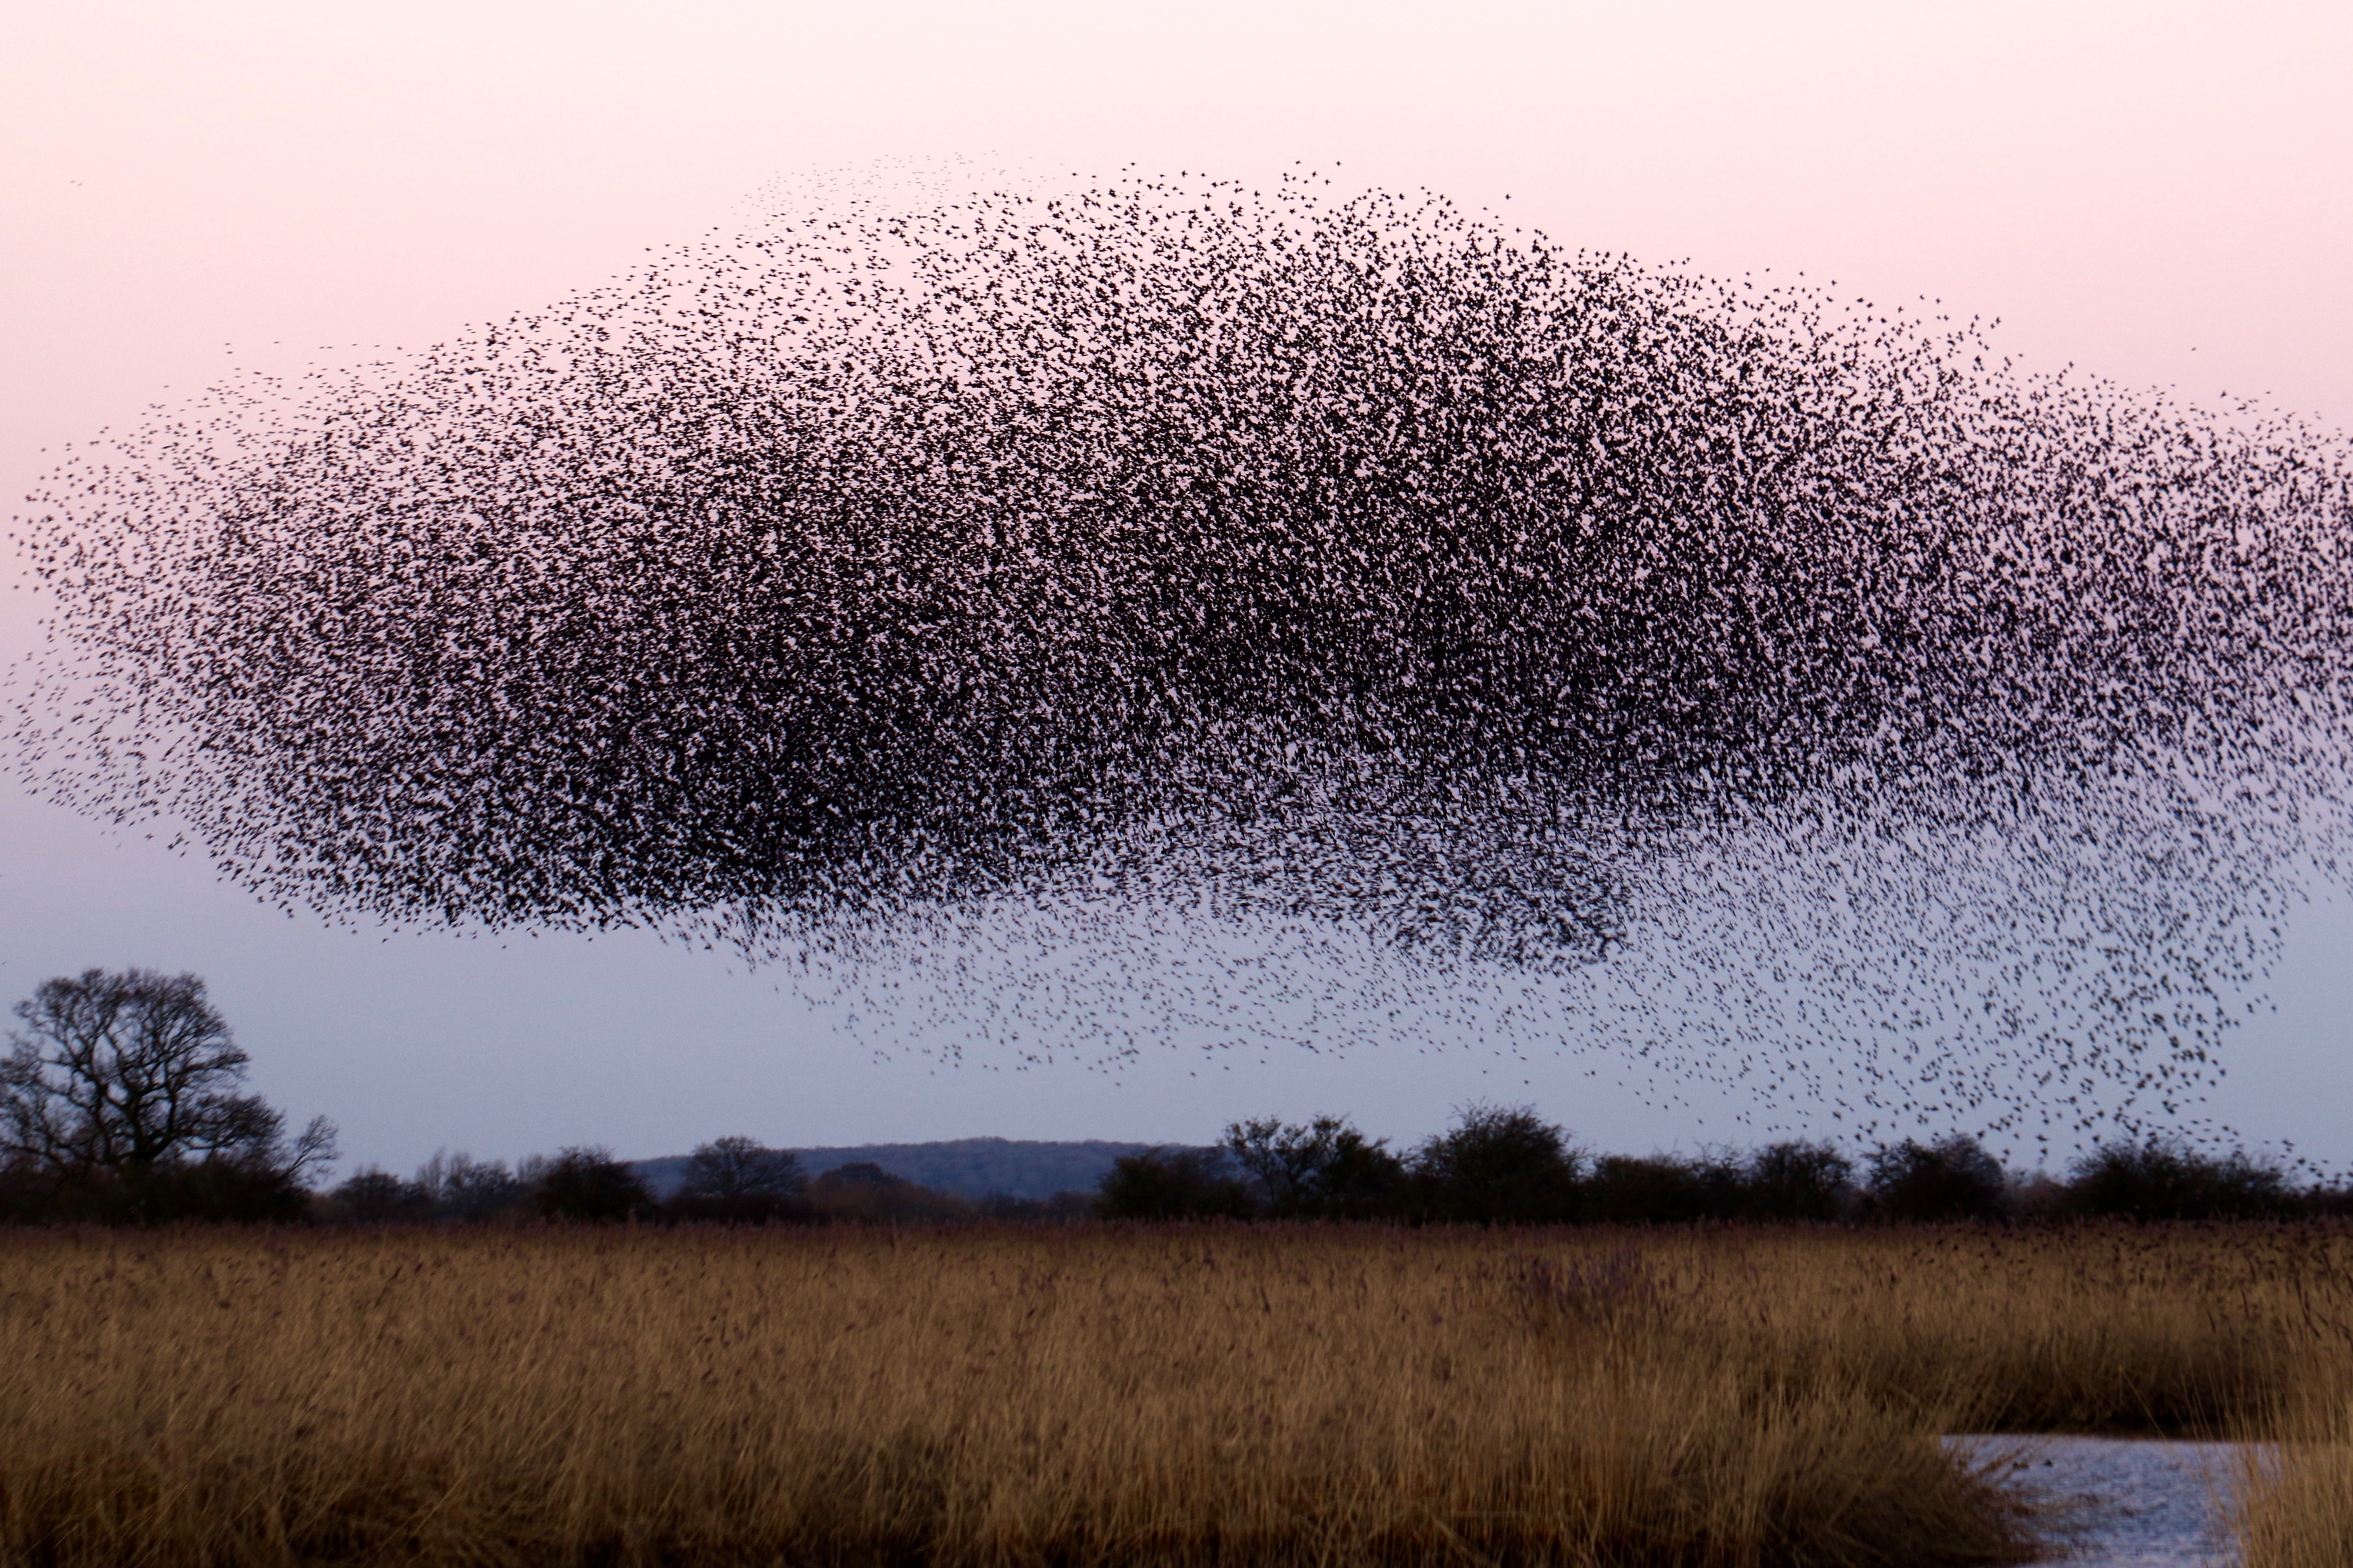
\includegraphics[width=\textwidth, keepaspectratio]{images/flock_image.jpeg}
\end{column}
\end{columns}
\end{minipage}
\end{frame}

\section{The Model}
\begin{frame}{Assumptions}
\begin{itemize}
  \item Convergence to a global critical state
  \vspace{0.5cm}
  \item Global interaction between birds
  \vspace{0.5cm}
  \item Interaction depending on visual perception
\end{itemize}
\end{frame}
\begin{frame}{Weighting Function}
	\begin{equation}
		v_i(t+h)-v_i(t)=h\sum_{j=1}^k a_{ij}(v_j(t)-v_i(t))\nonumber
	\end{equation}
  \vspace{1cm}
	\begin{equation}
		a_{ij}=\eta(x_i,x_j)=\frac{H}{(\sigma^2+\left\Vert x_i - x_j \right\Vert^2)^{\beta}}\nonumber
	\end{equation}
\end{frame}
\begin{frame}{Complex Network Theory}
	\begin{itemize}
		\item Adjacency matrix $A_x = \lbrace a_{ij}\rbrace=\bigg\lbrace\frac{H}{(\sigma^2+\left\Vert x_i - x_j \right\Vert^2)^{\beta}}\bigg\rbrace\nonumber$
		\vspace{0.5cm}
		\item Degree matrix $D_x = diag(d_1,...d_k) \text{, where } d_i=\bigg(\sum_{j\leq k}a_{ij}\bigg)v$
		\vspace{0.5cm}
		\item Laplacian matrix $L_x = D_x - A_x$
	\end{itemize}
\end{frame}
\begin{frame}{Discrete and Continuous Case}
	\begin{minipage}[0.95\textheight]{\textwidth}
	\begin{columns}[T]
	\begin{column}{0.5\textwidth}
		\begin{align}
			&x(t+h) = x(t) + hv(t)\nonumber\\
			&v(t+h) = (Id -hL_x)v(t)\nonumber
		\end{align}
	\end{column}
	\begin{column}{0.5\textwidth}
		\begin{align}
			&\dot{x} = v\nonumber\\
			&\dot{v} = -L_xv\nonumber
		\end{align}
	\end{column}
	\end{columns}
	\end{minipage}
\end{frame}

\section{Results}
\begin{frame}{Representative convergence}
	\begin{minipage}[0.95\textheight]{\textwidth}
	\begin{columns}[T]
	\begin{column}{0.50\textwidth}
	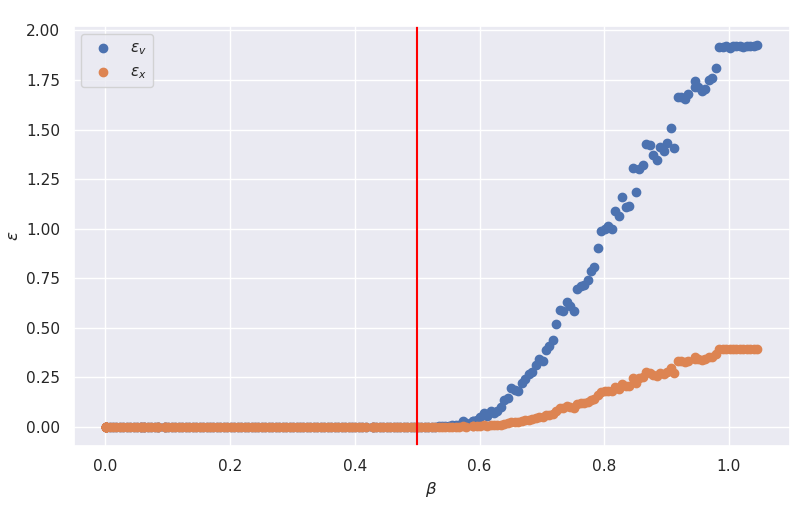
\includegraphics[width=\textwidth, keepaspectratio]{images/N100_sigma1.png}
	\end{column}
	\begin{column}{0.50\textwidth}
	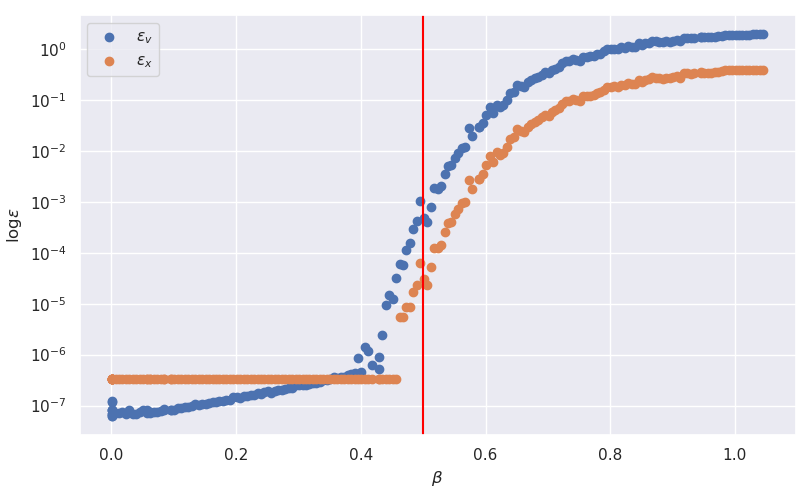
\includegraphics[width=\textwidth, keepaspectratio]{images/N100_sigma1log.png}
	\end{column}
	\end{columns}
	\end{minipage}
	\begin{center}
		Parameters: $k=100$, $\sigma=1$, \# iterations fixed
	\end{center}
\end{frame}
\begin{frame}{Influence of $\sigma$}
	\begin{minipage}[0.95\textheight]{\textwidth}
	\begin{columns}[T]
	\begin{column}{0.50\textwidth}
	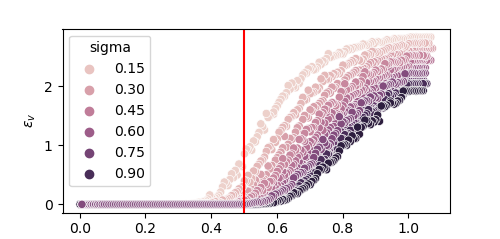
\includegraphics[width=\textwidth, keepaspectratio]{images/N100_sigmaA.png}
	\end{column}
	\begin{column}{0.50\textwidth}
	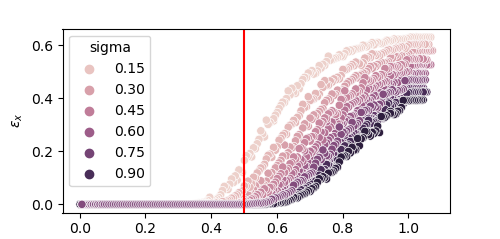
\includegraphics[width=\textwidth, keepaspectratio]{images/N100_sigmaAX.png}
	\end{column}
	\end{columns}
	\end{minipage}
	\begin{center}
		Parameters: $k=100$, $\sigma$ varying, \# iterations fixed
	\end{center}
\end{frame}
\begin{frame}{Influence of $k$}
	\begin{minipage}[0.95\textheight]{\textwidth}
	\begin{columns}[T]
	\begin{column}{0.50\textwidth}
	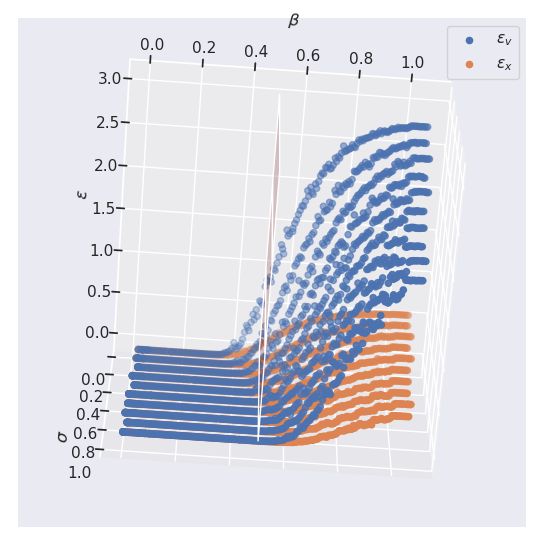
\includegraphics[width=\textwidth, keepaspectratio]{images/N100_3d.png}
	\end{column}
	\begin{column}{0.50\textwidth}
	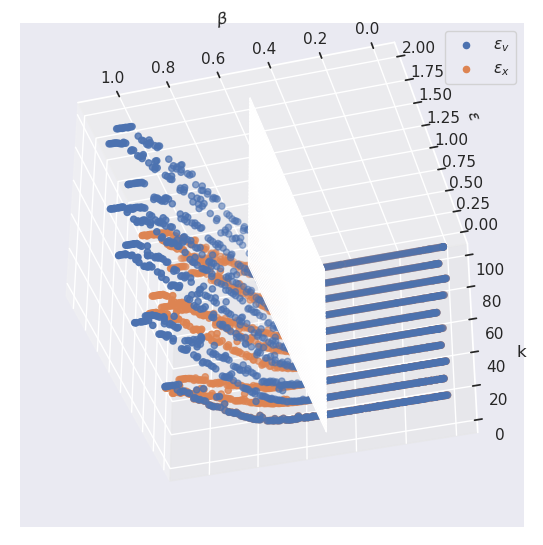
\includegraphics[width=\textwidth, keepaspectratio]{images/sigma1_3d.png}
	\end{column}
	\end{columns}
	\end{minipage}
\end{frame}
\begin{frame}{Combined 3D plots}
	\begin{minipage}[0.95\textheight]{\textwidth}
	\begin{columns}[T]
	\begin{column}{0.50\textwidth}
	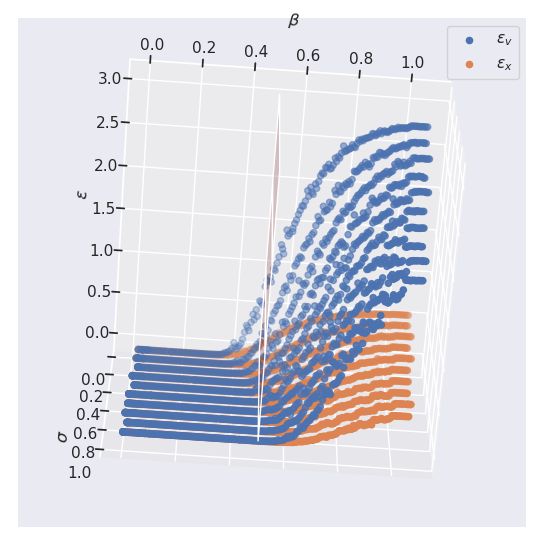
\includegraphics[width=\textwidth, keepaspectratio]{images/N100_3d.png}
	\end{column}
	\begin{column}{0.50\textwidth}
	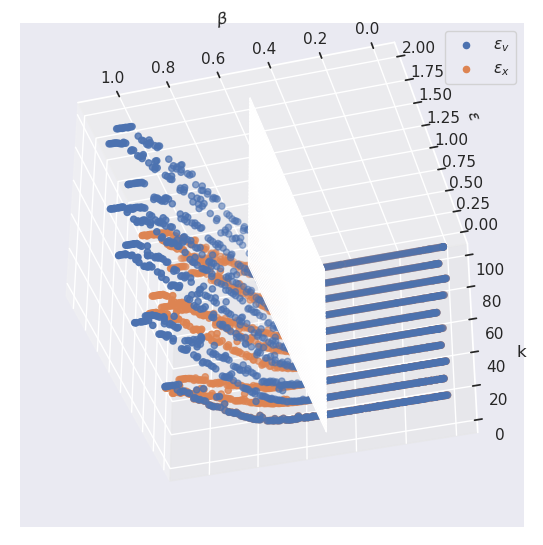
\includegraphics[width=\textwidth, keepaspectratio]{images/sigma1_3d.png}
	\end{column}
	\end{columns}
	\end{minipage}
	\begin{center}
		Parameters: $k$, $\sigma$ varying, \# iterations fixed
	\end{center}
\end{frame}

\end{document}